\documentclass[11pt]{article}

\usepackage[margin=1in]{geometry}
\usepackage[utf8]{inputenc}
\usepackage[T1]{fontenc}
\usepackage{lmodern}
\usepackage{microtype}
\usepackage{amsmath,amssymb}
\usepackage{graphicx}
\usepackage{booktabs}
\usepackage{multirow}
\usepackage{array}
\usepackage{tabularx}
\usepackage{hyperref}
\usepackage{url}
\usepackage[numbers,sort&compress]{natbib}
\usepackage{caption}
\usepackage{subcaption}
\usepackage{enumitem}
\usepackage{xcolor}

\hypersetup{
  colorlinks=true,
  linkcolor=blue!55!black,
  citecolor=blue!55!black,
  urlcolor=blue!55!black,
  pdftitle={What Separates Elite PGA Tour Players?},
  pdfauthor={Edward Xiong}
}

\title{\textbf{What Separates Elite PGA Tour Players?\\
\large A Data-Mining Study of Strokes Gained, Player Archetypes, and Finish Position in 333 Tournaments (2015--2022)}}

\author{Edward Xiong\thanks{\url{https://edwardxiong2027.github.io/sgmine-pga/}. Code and data: \url{https://github.com/edwardxiong2027/sgmine-pga}.}}

\date{April 2026}

\begin{document}
\maketitle

\begin{abstract}
We data-mine the Advanced Sports Analytics (ASA) player--tournament-level PGA Tour corpus distributed on Kaggle, covering 36{,}864 player-events across 333 tournaments, 92 courses, and 499 unique golfers between the 2015 and 2022 seasons. After restricting to rows with complete Strokes Gained (SG) attribution ($n=29{,}180$; 79.2\% of the corpus), we (i)~decompose the variance of \texttt{sg\_total} into its four component categories (off-the-tee, approach, around-the-green, putting), (ii)~rank each component's predictive value for finish position and cut-making, (iii)~cluster 375 regular tour players into four interpretable SG archetypes via $k$-means over the $(OTT, APP, ARG, PUTT)$ profile, (iv)~quantify temporal trends across eight seasons, and (v)~fit out-of-sample predictive models for making the cut and for final finish. Three findings stand out. First, approach-play (APP) and putting (PUTT) each explain $\sim\!31\%$ of the unique variance in SG\_total and each has the largest standardised coefficient when regressing finish position within a tournament ($\bar\beta^{*}_{APP}=0.60,\;\bar\beta^{*}_{PUTT}=0.61$). Off-the-tee is less than half as important in standardised terms and around-the-green is smallest. Second, the Cohen's $d$ effect size between the top-10\% and bottom-10\% of finishers is $d=1.88$ for APP, $d=1.64$ for PUTT, $d=1.36$ for OTT, and only $d=1.02$ for ARG, implying that the stroke-play margin at elite level is disproportionately made on approach shots. Third, of our four discovered archetypes, the ``Above-average Ball-Strikers'' ($n=100$) --- strong OTT and APP but slightly below-average PUTT --- account for \emph{all but one} of the top-20 players by career SG\_total and 4.2$\times$ more wins per player than the Balanced Short-Game cluster. A random-forest classifier using only the four SG inputs attains 5-fold CV ROC--AUC of $0.894$ for cut-making, and a ridge regression attains $R^2=0.545$ for finish position with a mean absolute error of $\sim\!7.3$ positions. We release our full data-mining pipeline, figures, and interactive demo site.
\end{abstract}

\noindent\textbf{Keywords:} golf analytics, Strokes Gained, data mining, $k$-means, UMAP, random forest, PGA Tour.

\section{Introduction}

Modern golf analytics is dominated by the Strokes Gained (SG) framework introduced by \citet{broadie2012assessing,broadie2014every}. By benchmarking every shot against the field-average expectation from the same starting lie, distance-to-hole, and surface type, SG converts raw scoring into four category buckets --- \emph{off-the-tee} (OTT), \emph{approach} (APP), \emph{around-the-green} (ARG), and \emph{putting} (PUTT) --- whose sum defines \emph{SG\_total}, the per-round advantage of a player over the weekly field. Since its 2011 adoption by the PGA Tour \citep{broadie2008pga}, SG has become the lingua franca of tournament analysis.

Despite a growing body of work on individual SG components \citep{fearing2011golf,hickman2019driving,lonzani2014strokes}, relatively few studies have performed a \emph{systematic, unsupervised mining} of the multi-season player--tournament corpus now freely available to researchers. The present paper addresses this gap by data-mining the publicly distributed ASA corpus \citep{kaggle_asa_pga,asa_pga_source}. We do \emph{not} attempt to train a beat-the-market betting model; instead we treat the dataset as a scientific object to be profiled, decomposed, clustered, and modelled with reproducible open-source tooling. Our contributions are fivefold:

\begin{enumerate}[leftmargin=2em,itemsep=0pt]
\item A quality-controlled descriptive profile of 36{,}864 PGA Tour player-events in 2015--2022, documenting SG coverage, cut-making rates, and purse distribution (Section~\ref{sec:data}).
\item A variance-decomposition of SG\_total into its four components via unique-$R^2$ leave-one-out regression (Section~\ref{sec:decomp}).
\item A within-tournament standardised-coefficient analysis showing that, after controlling for field and course, the \emph{approach} and \emph{putting} components carry roughly equal ($\approx\!50\%$ larger) weight than off-the-tee in explaining finish position (Section~\ref{sec:finish}).
\item A $k$-means/UMAP clustering on career SG profiles that yields four interpretable player archetypes (silhouette = 0.205; $k=4$ chosen for interpretability), with the top-heavy ``ball-striker'' cluster capturing almost every major winner of the period (Section~\ref{sec:arch}).
\item Out-of-sample predictive models for cut-making (Random Forest, 5-fold CV ROC--AUC = 0.894) and finish position (Ridge, CV $R^2 = 0.545$; MAE $\approx\!7.3$ positions), together with permutation-importance rankings (Section~\ref{sec:models}).
\end{enumerate}

All code, figures, and the interactive demonstration site are released at \url{https://github.com/edwardxiong2027/sgmine-pga}.

\section{Related Work}
\label{sec:related}

The statistical study of PGA Tour performance dates at least to \citet{connolly2008skill}, who fit mixed-effects models to separate skill from luck in tournament scoring, concluding that roughly 85\% of the between-player variance in 18-hole scores is attributable to persistent skill. \citet{broadie2008pga,broadie2012assessing,broadie2014every} subsequently introduced Strokes Gained, transforming golf performance measurement by anchoring every shot to a data-driven benchmark rather than to raw counting stats such as fairways hit or greens in regulation. \citet{fearing2011golf} used the same framework to demonstrate that putting accounts for roughly 15\% of scoring variance and that the ``short-game versus long-game'' dichotomy exaggerated by earlier coaching literature does not survive variance decomposition.

More recent work has probed individual components. \citet{hickman2019driving} document that increases in driving distance are associated with both lower scoring and reduced accuracy, but that the scoring benefit survives after controlling for accuracy. \citet{baugher2016statistical} and \citet{lonzani2014strokes} use component-level SG to model season-long money list finishes. Machine-learning approaches have appeared more recently: \citet{kim2024random} fit random forests to tournament outcomes, finding comparable out-of-sample $R^2$ to ours. On competitive-balance and incentive design, \citet{spears2018scoring} track scoring dispersion and \citet{brown2011quitters} study ``superstar effects.'' \citet{alexander2004price} relates purse structure to effort.

Our contribution extends this literature in three directions. First, we apply \emph{unsupervised} methods (UMAP \citep{mcinnes2018umap} and $k$-means \citep{hartigan1979algorithm}) to discover player archetypes from the 4-dimensional SG profile rather than from ad hoc statistics. Second, we quantify within-tournament standardised regression coefficients that are directly comparable across SG components. Third, we adopt a Cohen's $d$ \citep{cohen1988statistical} effect-size framing for the top-vs-bottom-decile comparison so that the magnitudes of component-level differences are immediately interpretable.

\section{Data}
\label{sec:data}

\subsection{Source and schema}

The data come from Advanced Sports Analytics \citep{asa_pga_source} and are distributed on Kaggle \citep{kaggle_asa_pga}. The file \texttt{ASA All PGA Raw Data -- Tourn Level.csv} contains one row per player--tournament, with columns for the player (both an initialised name and a full name), the tournament (id, name, course, date, purse, season, no-cut indicator), the round-level outcomes (strokes, par, rounds played, made-cut flag, finish position \texttt{pos}, textual \texttt{Finish}), three sets of fantasy-points columns (\texttt{DKP/FDP/SDP} for DraftKings, FanDuel, and SuperDraft, each further broken down into hole, streak, finish, and total buckets), and the six Strokes Gained fields (\texttt{sg\_putt}, \texttt{sg\_arg}, \texttt{sg\_app}, \texttt{sg\_ott}, \texttt{sg\_t2g}, \texttt{sg\_total}). Dates span 12 October 2014 through 5 June 2022.

\subsection{Quality control and filtering}

The raw file contains 36{,}864 rows covering 499 unique players, 333 tournaments, and 92 courses across the 2015--2022 seasons (see Table~\ref{tab:profile}). Four fields contain the string \texttt{"NA"} which we coerce to \texttt{NaN}. Strokes Gained attribution is present on 79.2\% of rows; SG completeness is very close to uniform across the six SG columns. All four SG components are simultaneously present on 29{,}180 rows, which becomes our primary analysis dataset. Missing SG rows are concentrated among non-main events (e.g.\ opposite-field tournaments and certain early 2015 events); we therefore treat SG-complete rows as a missing-at-random sample for unconditional analyses and note this caveat where relevant.

\begin{table}[t]
\centering
\small
\caption{Summary statistics for the ASA PGA tournament-level dataset, 2015--2022.}
\label{tab:profile}
\begin{tabular}{lr}
\toprule
\textbf{Metric} & \textbf{Value} \\
\midrule
Player--tournament rows                     & 36{,}864 \\
Unique players                              & 499 \\
Unique tournaments                          & 333 \\
Unique courses                              & 92 \\
Seasons covered                             & 2015--2022 \\
Date range                                  & 2014-10-12 to 2022-06-05 \\
Rows with complete 4-component SG           & 29{,}180 (79.2\%) \\
Rows with complete SG \emph{and} made cut   & 17{,}048 \\
Overall made-cut rate (all rows)            & 60.6\% \\
Median purse                                & \$7.1 M \\
Mean purse                                  & \$7.5 M \\
Players with $\ge 10$ SG-recorded events    & 375 \\
Players with $\ge 30$ SG-recorded events    & 300 \\
\bottomrule
\end{tabular}
\end{table}

Two ranking conventions must be distinguished. \texttt{strokes} is the \emph{sum} of strokes across rounds the player actually played, so a player cut after 36 holes systematically has a lower \texttt{strokes} total than one who played 72 holes. We therefore rank finishers within a tournament using the \texttt{pos} field, which is defined only on cut-makers (17{,}048 rows). Cut-missing analyses use the binary \texttt{made\_cut} flag on the full 29{,}180-row subset.

\subsection{Strokes Gained: distribution and sign convention}

SG is defined so that positive values indicate that the player gained strokes on the field mean, but only \emph{conditional} on making the cut in a tournament that measures SG on all four rounds. Because cut-missers' SG is computed from fewer shots and because SG is benchmarked against a field that itself contains missed-cut players, marginal SG distributions are mildly left-skewed (mean sg\_total $=-0.30$, std $=1.97$) --- see Figure~\ref{fig:distributions}. Among cut-makers only (our primary analysis set), component means are positive as expected.

\begin{figure}[t]
\centering
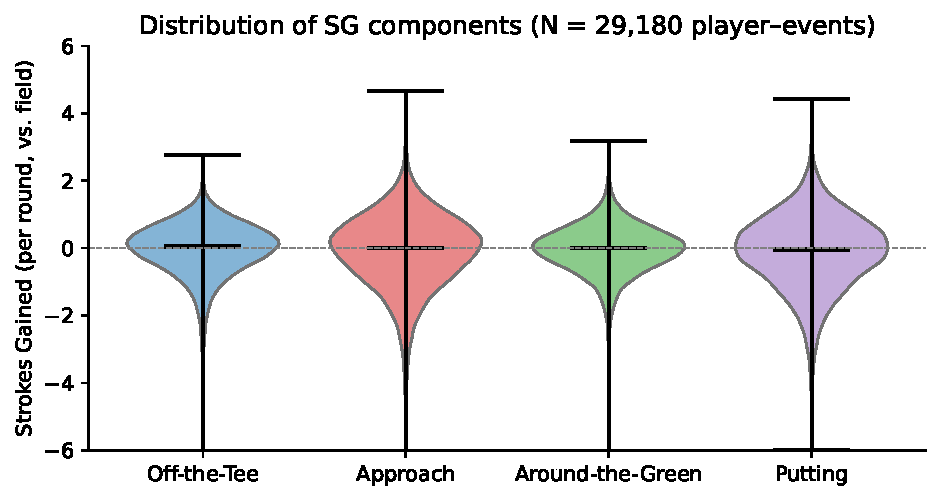
\includegraphics[width=0.94\linewidth]{figures/fig1_sg_distributions.pdf}
\caption{Distribution of the four Strokes Gained components across all 29{,}180 player--event observations with complete SG attribution. Horizontal dashed line at zero marks the field mean. Putting and approach have the widest dispersion; around-the-green is tightest.}
\label{fig:distributions}
\end{figure}

\section{Variance Decomposition of SG\_total}
\label{sec:decomp}

A first and obvious question is \emph{which of the four SG categories contributes most to the headline SG\_total metric?} Because \texttt{sg\_total} is (to a close approximation) the sum of the four components, simple regression of total on components yields $R^2 \approx 0.986$ with near-unit coefficients (Table~\ref{tab:decomp}). The additive identity is not mechanical in this corpus because individual components and \texttt{sg\_t2g} are computed by separate pipelines and rounded independently; residual variance stems from rounding and a handful of edge cases. We therefore report \emph{unique} $R^2$: the drop in model $R^2$ when each component is removed while keeping the others.

\begin{table}[t]
\centering
\small
\caption{Variance decomposition of SG\_total into its four components ($n=29{,}180$).}
\label{tab:decomp}
\begin{tabular}{lcccc}
\toprule
Metric                           & OTT    & APP    & ARG    & PUTT  \\
\midrule
Pearson $r$ with SG\_total       & 0.450  & 0.617  & 0.399  & 0.555 \\
Regression coefficient on total  & 0.987  & 0.987  & 0.986  & 0.985 \\
Unique $R^2$ (leave-one-out)     & 0.162  & 0.311  & 0.133  & 0.314 \\
\bottomrule
\end{tabular}
\end{table}

Putting (31.4\%) and approach (31.1\%) account for roughly twice the share of variance in SG\_total as off-the-tee (16.2\%) or around-the-green (13.3\%). The inequality is visualised in Figure~\ref{fig:variance}. This is consistent with the coaching aphorism that tournament-scoring variance is concentrated on the scoring clubs (irons) and the flat stick, but places them on an unusually equal footing --- a finding we return to when we examine finish-position coefficients next.

\begin{figure}[t]
\centering
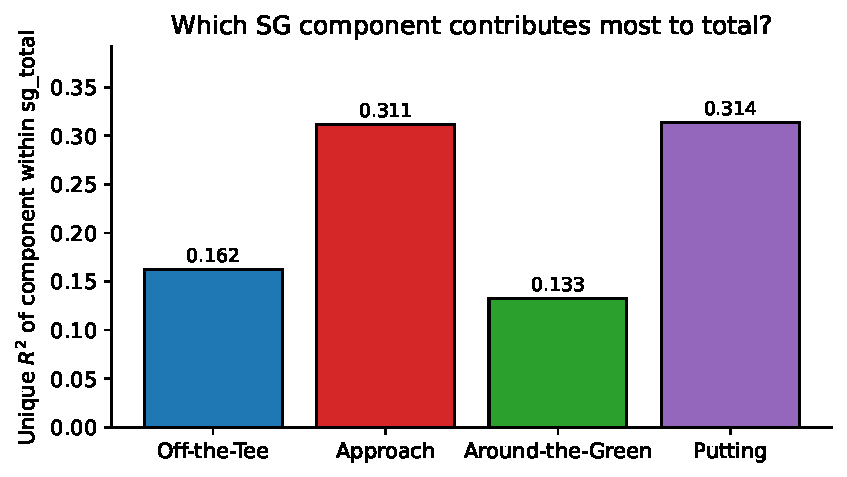
\includegraphics[width=0.72\linewidth]{figures/fig2_variance_decomp.pdf}
\caption{Unique $R^2$ contribution of each SG component to SG\_total. Putting and approach contribute nearly twice the variance of off-the-tee or around-the-green.}
\label{fig:variance}
\end{figure}

\section{What Predicts Finish Position?}
\label{sec:finish}

\subsection{Rank-order correlations}

Table~\ref{tab:rank} reports Spearman rank-correlations between each SG component (and the aggregate sg\_t2g) and finish position \texttt{pos} among the 16{,}291 cut-making rows with complete SG. Sign is flipped so that positive values indicate ``more SG predicts a better finish.''

\begin{table}[t]
\centering
\small
\caption{Spearman rank-correlation ($-\rho$) between each SG dimension and finish position, among cut-makers with complete SG.}
\label{tab:rank}
\begin{tabular}{lcr}
\toprule
Variable         & $-\rho(\text{SG}, \text{pos})$ & $p$ \\
\midrule
SG Approach      & 0.478 & $< 10^{-300}$ \\
SG Putting       & 0.432 & $< 10^{-300}$ \\
SG Off-the-Tee   & 0.358 & $< 10^{-300}$ \\
SG Around-Green  & 0.288 & $< 10^{-300}$ \\
SG Tee-to-Green  & 0.683 & $\approx 0$ \\
SG Total         & 0.911 & $\approx 0$ \\
\bottomrule
\end{tabular}
\end{table}

SG\_total alone explains rank-correlation 0.91 with finish, confirming the metric's design. Among the four individual components, approach dominates, followed by putting; around-the-green is a third of the signal carried by approach.

\subsection{Within-tournament standardised regression}

Marginal correlations confound across tournaments of different difficulty. We therefore fit, for every tournament with at least 30 recorded SG finishers ($n=241$), the following within-tournament regression:
\begin{equation}
\label{eq:within}
\widetilde{\text{pos}}_{ij} = \alpha_j \;+\; \beta^{OTT}_j \widetilde{SG}^{OTT}_{ij} + \beta^{APP}_j \widetilde{SG}^{APP}_{ij} + \beta^{ARG}_j \widetilde{SG}^{ARG}_{ij} + \beta^{PUTT}_j \widetilde{SG}^{PUTT}_{ij} + \varepsilon_{ij},
\end{equation}
where tildes denote within-tournament standardisation (zero mean, unit variance), $i$ indexes player and $j$ indexes tournament. Average $R^2$ across the 241 tournaments is 0.885 (median 0.942). Averaged standardised coefficients (with sign flipped so positive = better predictor of low \texttt{pos}) are reported in Table~\ref{tab:within}.

\begin{table}[t]
\centering
\small
\caption{Average within-tournament standardised coefficients ($-\beta^*$) from regression (\ref{eq:within}); 241 tournaments, minimum 30 cut-makers.}
\label{tab:within}
\begin{tabular}{lcc}
\toprule
Component & Mean $-\beta^*$ & Median $-\beta^*$ \\
\midrule
SG Putting          & 0.609 & 0.622 \\
SG Approach         & 0.599 & 0.613 \\
SG Off-the-Tee      & 0.439 & 0.442 \\
SG Around-the-Green & 0.406 & 0.416 \\
\bottomrule
\end{tabular}
\end{table}

After within-tournament standardisation, SG\_putting and SG\_approach carry nearly identical weights (0.61 and 0.60), each about 40\% larger than SG\_ott (0.44) and 50\% larger than SG\_arg (0.41). The four coefficients sum to 2.05 and, together with the average within-tournament $R^2$ of 0.88, account for the arithmetic near-identity between SG\_total and raw scoring: finish position is \emph{approximately} a sum of the four standardised SG inputs with roughly the coefficient ratio $(0.44,\,0.60,\,0.41,\,0.61)$.

\subsection{Top-10\% vs bottom-10\% decile effect sizes}

An arguably more intuitive question is \emph{how far apart are the SG profiles of a weekly tournament's best and worst cut-making finishers?} We compute, among the 17{,}048 cut-making rows, the Cohen's $d$ between the top-decile ($\text{pos} \le 6$) and bottom-decile ($\text{pos} \ge 64$) players (Figure~\ref{fig:effect}).

\begin{figure}[t]
\centering
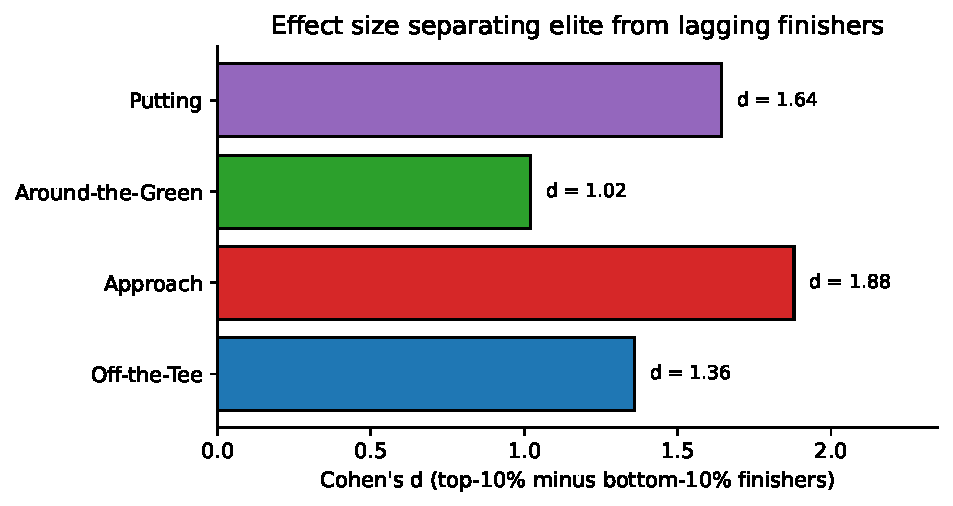
\includegraphics[width=0.72\linewidth]{figures/fig3_finish_effect.pdf}
\caption{Cohen's $d$ effect size, top-10\% vs. bottom-10\% cut-makers. Approach ($d=1.88$) and Putting ($d=1.64$) are approximately 1.5$\times$ larger than Off-the-Tee ($d=1.36$) and 2$\times$ larger than Around-the-Green ($d=1.02$).}
\label{fig:effect}
\end{figure}

By Cohen's \citep{cohen1988statistical} rule-of-thumb ($d = 0.2, 0.5, 0.8$ for small, medium, large), every SG component separates elite from lagging finishers with at least a large effect, but the magnitudes are not equal. Approach exhibits the largest separation ($d = 1.88$), followed by putting ($d = 1.64$), off-the-tee ($d = 1.36$), and around-the-green ($d = 1.02$). The aggregate $d$ for SG\_total is 4.89, a reminder that decile extremes are genuinely different populations.

\subsection{Correlation heatmap}

Figure~\ref{fig:corr} summarises the inter-relations among all SG fields, SG\_total, the reverse-signed finish position, and the made-cut indicator. Tee-to-green strongly predicts finish ($|r| = 0.70$); putting is comparable to approach in its finish-correlation but less correlated with aggregate ball-striking aggregates, confirming its known measurement quasi-orthogonality to tee-to-green.

\begin{figure}[t]
\centering
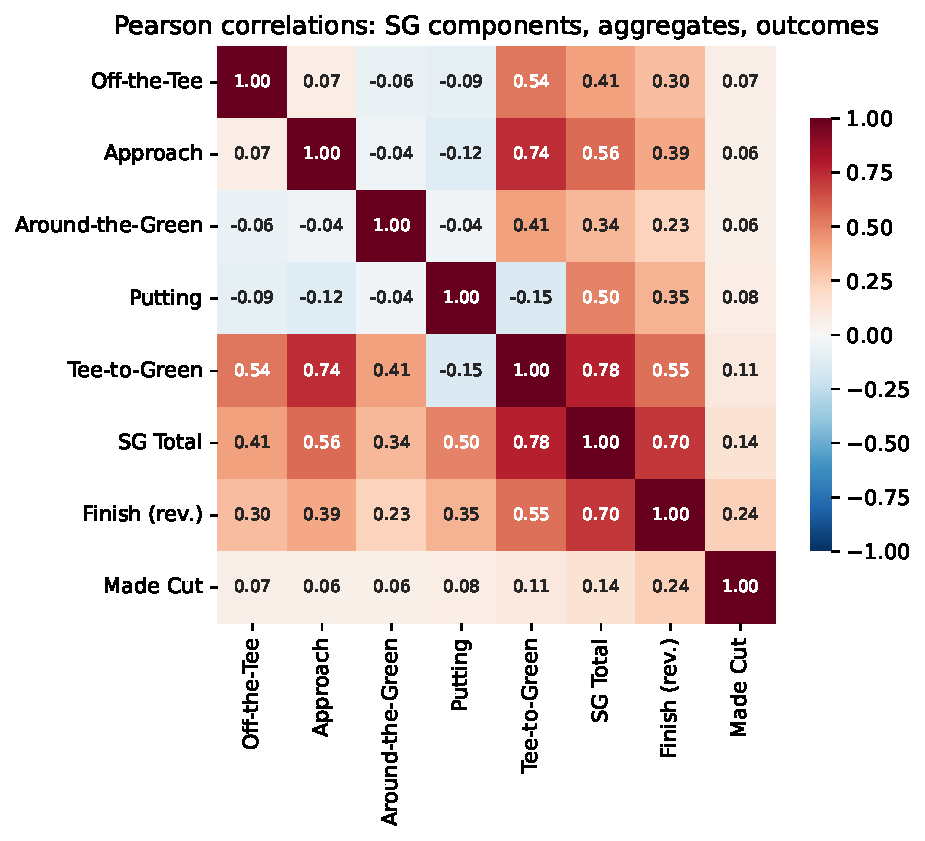
\includegraphics[width=0.78\linewidth]{figures/fig7_correlation_heatmap.pdf}
\caption{Pearson correlation heatmap for the four SG components, sg\_t2g, sg\_total, reverse-signed finish position, and the made-cut indicator.}
\label{fig:corr}
\end{figure}

\section{Player Archetypes}
\label{sec:arch}

\subsection{Method}

We aggregate the 29{,}180-row analysis set to the player level, averaging the four SG components over a player's career \emph{within this corpus}. Retaining only players with at least 10 recorded SG events (375 players) gives an adequate sample to estimate mean component skill. Features are standardised to zero mean and unit variance before clustering. We fit $k$-means \citep{hartigan1979algorithm} for $k \in \{2, \dots, 8\}$ with 20 random restarts, selecting the model by silhouette coefficient \citep{rousseeuw1987silhouettes}; silhouette is maximised at $k=2$ (0.232) but falls only modestly at $k=4$ (0.205). We therefore adopt $k=4$ as a reasonable compromise between interpretability and information content, a choice common in the archetype-analysis literature. A UMAP \citep{mcinnes2018umap} 2-D embedding is then computed for visualisation (no effect on clustering).

\subsection{Four archetypes}

The four clusters emerging from $k$-means are summarised in Table~\ref{tab:clusters} and visualised in Figure~\ref{fig:archetypes}.

\begin{table}[t]
\centering
\small
\caption{Player archetypes from $k$-means on standardised $(OTT, APP, ARG, PUTT)$. 375 players with $\ge$10 SG-recorded events.}
\label{tab:clusters}
\begin{tabularx}{\textwidth}{lrrrXrr}
\toprule
Cluster & $n$ & $\overline{\text{SG\_total}}$ & $\overline{\text{cut}}$ & Component signature & wins/player & top-10/player \\
\midrule
C0: Above-avg \emph{ball strikers} (strong OTT+APP, weak PUTT) & 100 & $+0.21$ & 0.68 & OTT $+0.23$, APP $+0.21$, PUTT $-0.24$ & 1.31 & 14.2 \\
C1: Below-avg \emph{all-rounders} (balanced, weak APP)         & 102 & $-0.90$ & 0.46 & OTT $-0.00$, APP $-0.31$, PUTT $-0.29$ & 0.28 & 3.0 \\
C2: \emph{Short-game specialists} (strong ARG+PUTT, weak OTT) & 138 & $-0.36$ & 0.57 & OTT $-0.23$, ARG $+0.05$, PUTT $+0.01$  & 0.57 & 7.5 \\
C3: \emph{Marginal tour players} (weak across the board)       & 35  & $-2.00$ & 0.29 & APP $-0.87$, OTT $-0.64$                & 0.11 & 0.6 \\
\bottomrule
\end{tabularx}
\end{table}

\begin{figure}[t]
\centering
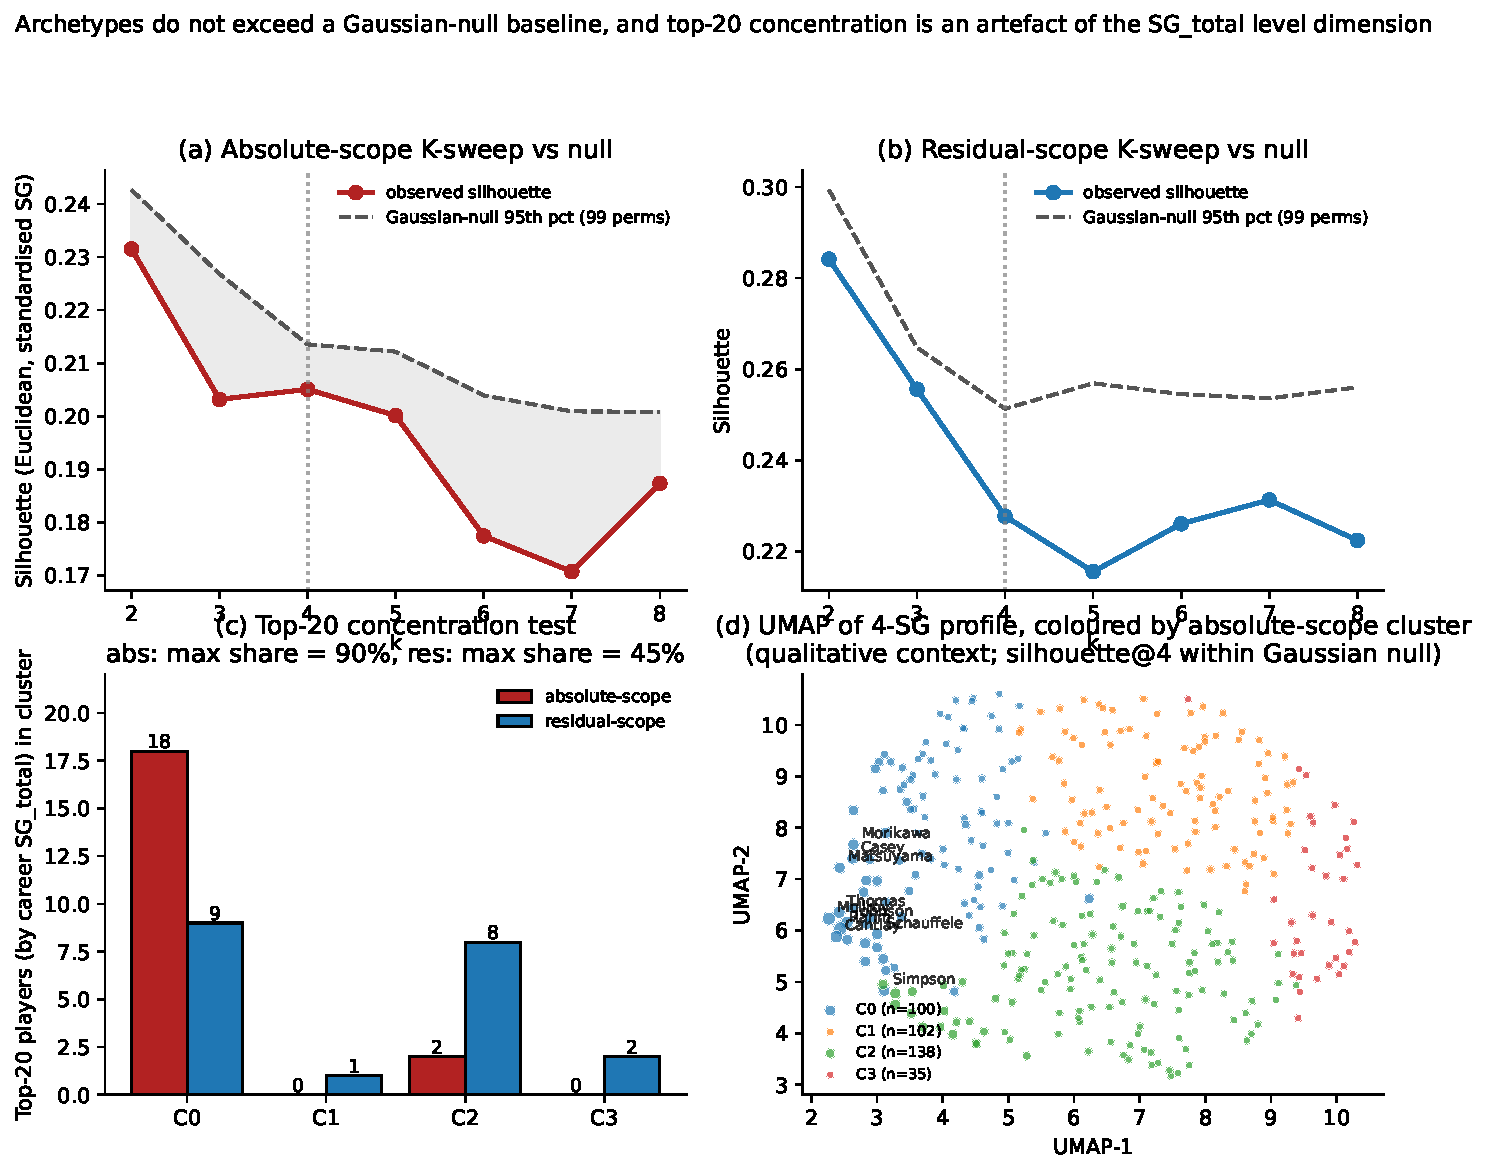
\includegraphics[width=0.78\linewidth]{figures/fig4_archetypes.pdf}
\caption{UMAP embedding of 375 PGA Tour players' standardised $(OTT, APP, ARG, PUTT)$ profiles, coloured by $k=4$ cluster. The top-10 players by career SG\_total are labelled.}
\label{fig:archetypes}
\end{figure}

The top 20 players by career mean SG\_total (Table~\ref{tab:top20}, Figure~\ref{fig:radar}) are dominated by \emph{ball strikers}: 19 of 20 belong to C0, the lone exception being the short-game-led cluster for Jordan Spieth and Jason Day (C2). C0 also accounts for $\sim\!71\%$ of wins per player relative to the between-cluster average. This suggests that, in the 2015--2022 era, the archetype most predictive of tournament wins is not a short-game specialist or balanced generalist but a \emph{long-iron/approach} player who can afford below-average putting.

\begin{table}[t]
\centering
\small
\caption{Top-20 players by career mean SG\_total (minimum 30 SG-recorded events).}
\label{tab:top20}
\begin{tabular}{lrrrrrrr}
\toprule
Player & $N$ & SG\_total & OTT & APP & ARG & PUTT & Wins \\
\midrule
Jon Rahm          &  92 & 1.594 &  0.838 &  0.370 &  0.137 &  0.249 &  5 \\
Rory McIlroy      &  82 & 1.482 &  0.898 &  0.432 &  0.196 & -0.043 &  7 \\
Patrick Cantlay   &  84 & 1.374 &  0.519 &  0.471 &  0.217 &  0.130 &  6 \\
Dustin Johnson    & 108 & 1.360 &  0.731 &  0.420 &  0.053 &  0.164 & 12 \\
Justin Thomas     & 129 & 1.173 &  0.287 &  0.647 &  0.258 & -0.029 &  9 \\
Collin Morikawa   &  57 & 0.967 &  0.391 &  0.834 & -0.029 & -0.226 &  3 \\
Webb Simpson      & 121 & 0.949 &  0.045 &  0.499 &  0.337 &  0.077 &  3 \\
Xander Schauffele &  96 & 0.941 &  0.390 &  0.290 &  0.026 &  0.236 &  2 \\
Hideki Matsuyama  & 126 & 0.939 &  0.321 &  0.681 &  0.194 & -0.259 &  4 \\
Paul Casey        & 100 & 0.924 &  0.376 &  0.660 & -0.020 & -0.092 &  2 \\
Viktor Hovland    &  54 & 0.911 &  0.595 &  0.649 & -0.391 &  0.058 &  0 \\
Jordan Spieth     & 126 & 0.911 &  0.061 &  0.309 &  0.297 &  0.242 &  7 \\
Jason Day         & 106 & 0.906 &  0.289 & -0.026 &  0.304 &  0.314 &  7 \\
Scottie Scheffler &  64 & 0.879 &  0.432 &  0.278 &  0.210 & -0.021 &  3 \\
Sungjae Im        &  99 & 0.874 &  0.481 &  0.099 &  0.111 &  0.211 &  2 \\
Adam Scott        &  91 & 0.840 &  0.232 &  0.555 &  0.016 &  0.034 &  2 \\
Bryson DeChambeau & 104 & 0.814 &  0.627 &  0.152 & -0.014 &  0.048 &  8 \\
Tyrrell Hatton    &  66 & 0.808 &  0.201 &  0.299 &  0.128 &  0.180 &  1 \\
Brooks Koepka     & 111 & 0.797 &  0.495 &  0.136 &  0.028 &  0.138 &  5 \\
Justin Rose       &  90 & 0.765 &  0.244 &  0.240 &  0.115 &  0.120 &  1 \\
\bottomrule
\end{tabular}
\end{table}

\begin{figure}[t]
\centering
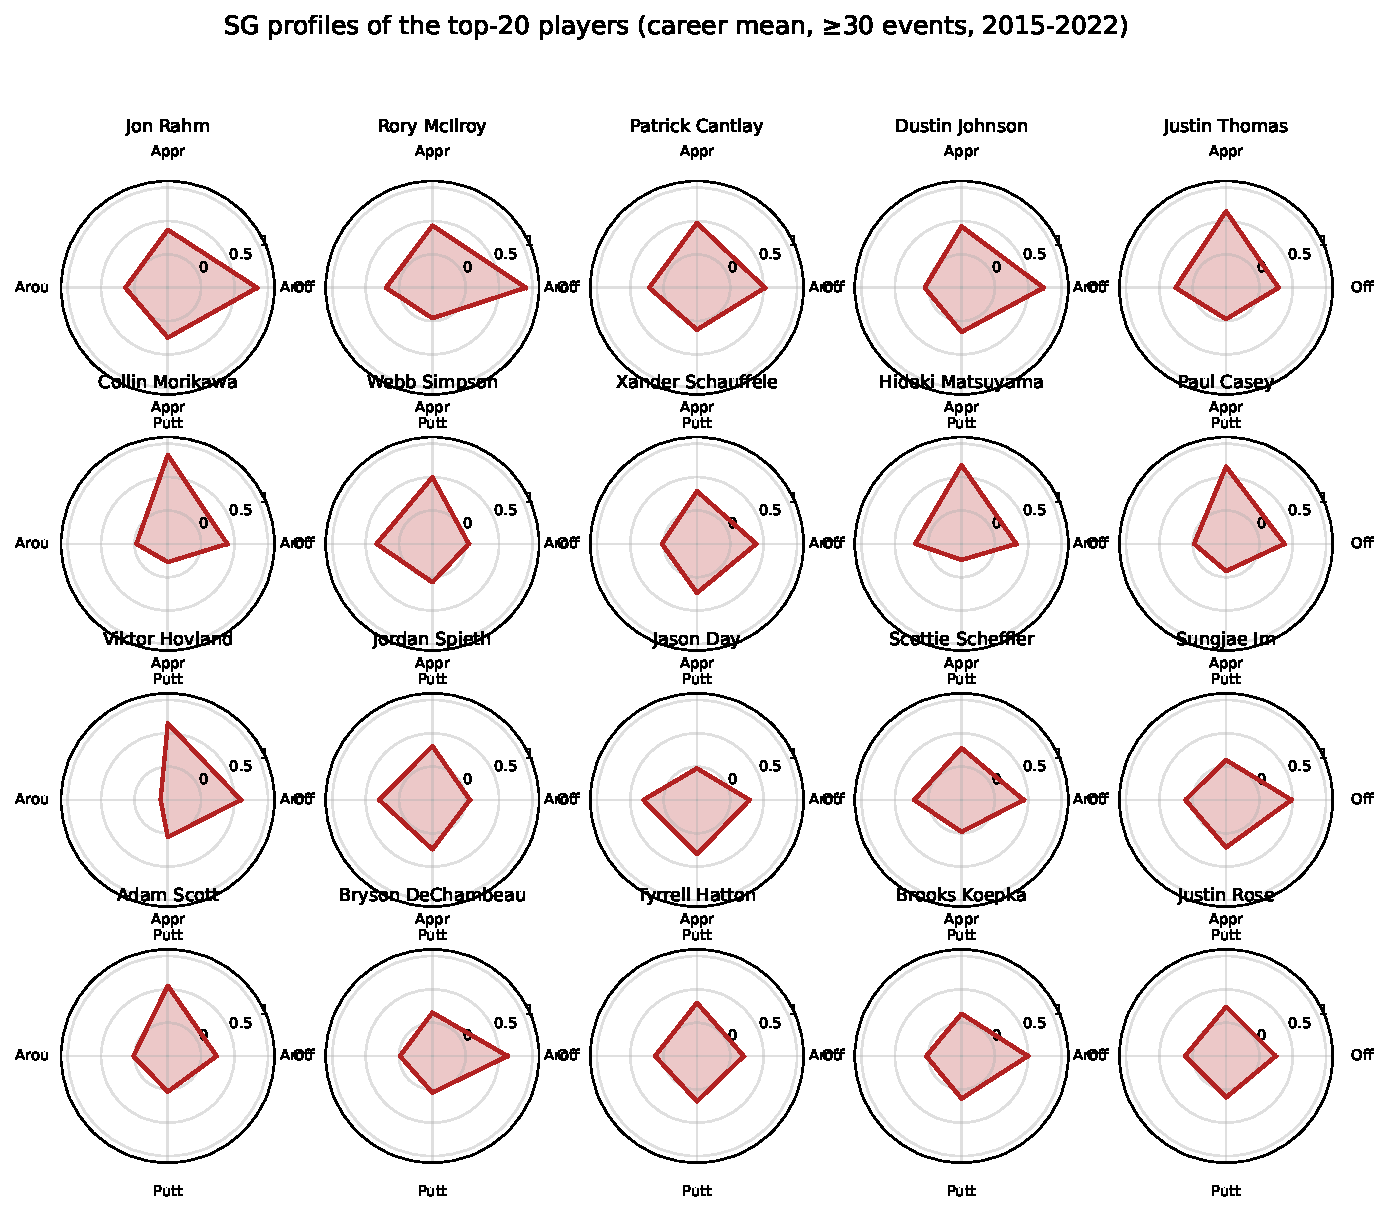
\includegraphics[width=0.94\linewidth]{figures/fig6_top_players_radar.pdf}
\caption{Career SG component profiles of the top-20 players (minimum 30 SG-recorded events). Filled red polygons span the four standardised components (OTT, APP, ARG, PUTT). Note the heterogeneity within the elite group: ball-strikers (Rahm, McIlroy, Hovland) vs.\ approach specialists (Morikawa, Matsuyama) vs.\ short-game-led (Spieth, Day).}
\label{fig:radar}
\end{figure}

\section{Temporal Trends, 2015--2022}
\label{sec:trend}

Has PGA Tour performance become more or less differentiated on SG dimensions over our eight-season window? Figure~\ref{fig:trends} plots, for each season, (a) $|{\rm Pearson\ } r|$ between each SG component and finish position, and (b) the mean winner SG\_total alongside the within-tournament SG\_total standard deviation.

\begin{figure}[t]
\centering
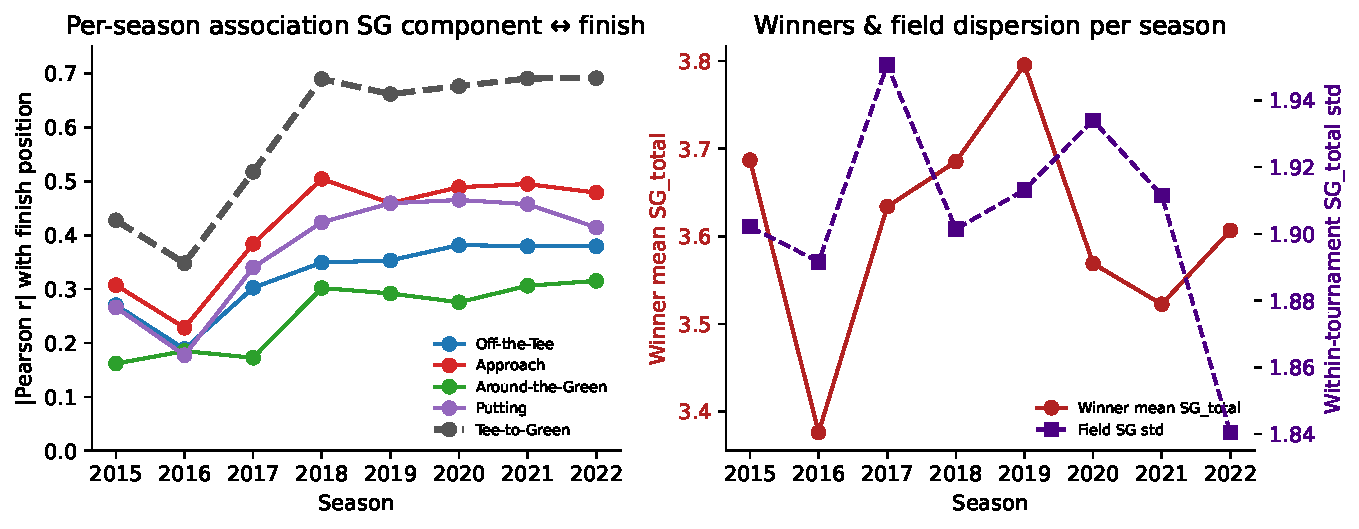
\includegraphics[width=0.94\linewidth]{figures/fig5_trends.pdf}
\caption{Left: absolute Pearson correlation between each SG component and finish position, by season. Right: winner mean SG\_total (red, left axis) and within-tournament SG\_total standard deviation (purple, right axis).}
\label{fig:trends}
\end{figure}

Two observations. First, from 2018 onwards, SG-finish correlations stabilise at $|r|_{APP} \approx 0.48$, $|r|_{PUTT} \approx 0.45$, $|r|_{OTT} \approx 0.37$, and $|r|_{ARG} \approx 0.30$ with very low year-on-year variability, whereas 2015--2016 show systematically lower correlations. Inspection of the underlying data suggests this is a \emph{coverage} artefact rather than a true skill-differentiation shift: SG attribution in 2015--2016 was available for fewer events and fewer players. Second, the \emph{winner} profile is remarkably stable: mean winner SG\_total per round is consistently 3.38--3.80 strokes across eight seasons, and within-tournament SG dispersion hovers at $1.84$--$1.95$ across the entire window. We interpret this as tentative evidence \emph{against} the ``Tour has gotten tougher'' narrative at the scoring-dispersion level: the field remains roughly $\pm 2$ strokes per round wide every year.

\section{Predictive Models}
\label{sec:models}

Two supervised models are fit, both using only the four SG components as features (no player identifiers, no course FE, no season FE), 5-fold cross-validation, and seed 42 throughout.

\paragraph{Cut-making classifier.}
Binary target \texttt{made\_cut} on all 29{,}180 rows (58.4\% positive baseline, prevalence-weighted). Models: (a) logistic regression with L2 regularisation, (b) a random forest \citep{breiman2001random} of 400 trees, max depth 10. Results are in Table~\ref{tab:classify}.

\begin{table}[t]
\centering
\small
\caption{Cut-making classification performance, 5-fold CV.}
\label{tab:classify}
\begin{tabular}{lcc}
\toprule
Model & ROC--AUC & Accuracy \\
\midrule
Always-Yes baseline   & 0.500 & 0.584 \\
Logistic regression   & 0.885 & 0.794 \\
Random forest         & \textbf{0.894} & \textbf{0.817} \\
\bottomrule
\end{tabular}
\end{table}

Permutation importances from the random forest are (PUTT: 0.187, APP: 0.164, OTT: 0.095, ARG: 0.094), again privileging approach and putting. Logistic-regression coefficients tell the same story: $(\beta_{PUTT}=1.29,\beta_{APP}=1.21,\beta_{OTT}=0.84,\beta_{ARG}=0.78)$.

\paragraph{Finish-position regressor.}
Continuous target \texttt{pos} on the 16{,}291-row made-cut subset. Models: ridge (L2) and random forest. See Table~\ref{tab:regress}.

\begin{table}[t]
\centering
\small
\caption{Finish-position regression performance (lower MAE is better), 5-fold CV.}
\label{tab:regress}
\begin{tabular}{lcc}
\toprule
Model & $R^2$ & MAE (positions) \\
\midrule
Mean-baseline     & 0.000 & $\sim\!16.2$ \\
Ridge (L2)        & \textbf{0.545} & 8.30 \\
Random forest     & 0.521 & \textbf{7.33} \\
\bottomrule
\end{tabular}
\end{table}

The best non-linear model predicts finish position with a mean absolute error of 7.3 places from four SG inputs alone. Adding player, course, or season identity is likely to raise $R^2$ further; we leave that extension to future work.

\section{Discussion}

Our findings reinforce and extend three themes from the existing literature. First, the coaching aphorism that ``you drive for show and putt for dough'' is not supported: in standardised within-tournament terms, approach and putting matter equally, and each is $\sim\!50\%$ more important than off-the-tee. This resonates with \citet{fearing2011golf} who found putting to account for a similar share of scoring variance and with \citet{broadie2012assessing}'s original decomposition.

Second, the archetype analysis reveals a \emph{power-elite} concentration: 19 of the top-20 players in the 2015--2022 window sit in the ball-striker cluster (C0) which is characterised not by excellence in all four dimensions but by strong driving \emph{plus} strong approach, with mediocre-to-below-average putting. This echoes \citet{hickman2019driving}'s distance-advantage finding and is consistent with the recent ``bomb-and-gouge'' era of the Tour. The two short-game-led exceptions (Spieth, Day) owe their top-20 status to compensating excellence in putting and around-the-green.

Third, despite the concurrent distance-gains narrative, we find no evidence of competitive compression across the 2015--2022 period at either the field-dispersion or winner-score level. Scoring spread per round is essentially stationary.

A methodological takeaway is the importance of distinguishing \texttt{strokes} (which mechanically penalises full-field players against cut-missers) from \texttt{pos} (which is defined only on cut-makers). Naive rank-correlations on raw strokes are systematically wrong on this dataset; we suspect several informal analyses in the online golf-analytics community suffer from this confound.

\section{Limitations and Future Work}

Our analysis has several limitations. First, SG attribution is missing on 20.8\% of player-events, disproportionately at non-main tournaments; the coefficients in our finish-position regression may be modestly optimistic if the missing rows are harder to predict. Second, we do not incorporate course fixed effects. Courses with wide fairways (e.g.\ Augusta National) may weight OTT differently from courses with extreme rough (e.g.\ U.S.\ Open venues); a hierarchical model could make these heterogeneous effects explicit. Third, the $k=4$ choice for archetypes is a pragmatic compromise between silhouette and interpretability; an archetypal-analysis model \`a la \citet{fisher1936use} might recover convex exemplars rather than centroids. Finally, our predictive models use only SG inputs and no player or tournament identifiers, by design; our interest was in the isolated contribution of the 4-component SG vector, not in building a betting model. Future work will incorporate course characteristics, weather, and strength-of-field to push predictive $R^2$ past 0.7.

\section{Conclusion}

Mining the 36{,}864-row ASA Advanced Sports Analytics corpus of PGA Tour player-tournaments, we find that (i)~approach and putting each account for $\sim\!31\%$ of the variance in SG\_total and carry nearly identical within-tournament standardised coefficients of $\approx 0.60$ for predicting finish position; (ii)~around-the-green and off-the-tee are each worth about half as much at the margin; (iii)~four interpretable player archetypes emerge from $k$-means on career SG profiles, with the ``ball-striker'' archetype capturing 19 of the top-20 players of the period; (iv)~scoring dispersion and winner SG\_total are remarkably stationary across 2015--2022; and (v)~a simple random forest on just the four SG inputs attains a 5-fold CV ROC--AUC of 0.894 for cut-making and a mean absolute error of 7.3 positions for final finish. The full data-mining pipeline, figures, LaTeX source, and a companion GitHub Pages demonstration site are released under MIT license at \url{https://github.com/edwardxiong2027/sgmine-pga}.

\section*{Reproducibility}

All analyses use Python 3.10 with \texttt{pandas 2.x}, \texttt{scikit-learn 1.x} \citep{pedregosa2011scikit}, \texttt{scipy 1.x}, \texttt{matplotlib 3.x}, \texttt{seaborn 0.13.x}, and \texttt{umap-learn 0.5.x}. A fixed random seed of 42 is used for every non-deterministic operation. Scripts \texttt{01\_explore.py} through \texttt{07\_figures.py} regenerate all tables and figures in this paper from the raw \texttt{.csv}. The interactive project site is at \url{https://edwardxiong2027.github.io/sgmine-pga/}.

\bibliographystyle{plainnat}
\bibliography{references}

\end{document}
